\documentclass[french]{report}
\usepackage[utf8]{inputenc}
\usepackage[T1]{fontenc}
\usepackage{latexsym}
\usepackage{amsfonts}
\usepackage{enumerate}
\usepackage{amsmath}
\usepackage{amsthm}
\usepackage{amssymb}
\usepackage{array}
\usepackage{enumitem}
\usepackage[french]{babel}
\usepackage{fancybox}
\usepackage{xcolor}
\usepackage{caption}
\usepackage{graphicx}
\usepackage{listings}
\usepackage{array}
\usepackage{float}
\usepackage{hyperref}

\usepackage[ruled,lined]{algorithm2e}


\AddThinSpaceBeforeFootnotes 
\FrenchFootnotes



\newtheorem{thm}{Théorème}[section] 
\newtheorem{lem}{Lemme}[section]
\newtheorem{prop}{Proposition}[section]
\newtheorem{defn}{Definition}[section]
\newtheorem{exmp}{Exemple}[section]
\newtheorem{algo}{Algorithme}[section]

\newcommand{\theoreme}[2]{\begin{thm}[#1] #2\end{thm}}
\newcommand{\definition}[2]{\begin{defn}[#1] #2 \end{defn}}
\newcommand{\proposition}[2]{\begin{prop}[#1] #2 \end{prop}}
\newcommand{\example}[2]{\begin{exmp}[#1] #2 \end{exmp}}
\newcommand{\preuve}[1]{\begin{proof} #1 \end{proof}}
\newcommand{\lemme}[2]{\begin{lem}[#1] #2 \end{lem}}

\newcommand{\D}{\mathbb{D}}
%\addto\captionsfrench{\def\proofname{\textcolor{thm_title}{\fontsize{11}{14}\selectfont Preuve}}}

%\newcommand{\preuve}[1]{\begin{proof} #1 \end{proof}}


\author{Esteban Foncoux}



\begin{document}

\begin{titlepage}

    \begin{figure}[h!]
        \begin{center}
            
\includegraphics[width=5cm]{unamur.png}
        \end{center}
    \end{figure}

    \begin{center}
        \textbf{\LARGE{UNIVERSITE DE NAMUR}} \\
        \vspace{0.5cm}
        \textbf{\LARGE{Faculté des Sciences}}
    \end{center}



    \vspace{1cm}

    \begin{center}

        \textrm{ \textbf{\LARGE{Étude des méthodes de recherche directe pour la calibration d’un modèle épidémiologique}}}


    \end{center}

    \vspace{0.5cm}

    \begin{center}
        \LARGE{ }
    \end{center}
    \vspace{3cm}


    \begin{center}
        \textbf{Mémoire présenté pour l'obtention\\du grade académique de master à finalité spécialisée en Data science } \\
        Esteban FONCOUX \\
        Juin 2024
    \end{center}


\end{titlepage}


\newpage
\chapter*{Résumé}

Ce mémoire a pour objectif l'étude des méthodes d’optimisation de recherche directe, en utilisant le logiciel open-source NOMAD\cite{Nomad} implémenté en \verb!C++!, pour la calibration d’un modèle épidémiologique. En effet, la calibration d'un modèle peut être extrêmement coûteuse en temps et en ressources et obtenir de nouvelles méthodes d'optimisation plus efficaces que celles utilisées actuellement peut être très utile.

L'objectif de ce mémoire est de construire des modèles épidémiologiques plus ou moins complexes afin de tester ces méthodes de recherche directe avec différents niveaux de complexité et comparer les résultats obtenus avec un algorithme de recherche aléatoire et ainsi conclure ou non de la viabilité de ces algorithmes lors de l'étape de calibration.

\chapter*{Abstract}
\tableofcontents
\newpage

\chapter*{Introduction}
\addcontentsline{toc}{chapter}{Introduction}

\chapter{Modèles épidémiologiques}

\section{L'épidémiologie}

L'ouvrage \textit{A dictionary of epidemilogy} \cite{ADictionaryofEpidemiology} définit l'épidémiologie comme \og l'étude de l’occurrence et la distribution des évènements, états et processus liés à la santé dans des populations spécifiques, y compris l'étude des déterminants qui influencent ces processus, et l'application de ces connaissances pour contrôler les problèmes de santé pertinents \fg.

Afin de clarifier cela, décomposons les différents termes de la définition. L'étude reprend plus globalement la surveillance, l'observation, le dépistage, la vérification d'hypothèses, la recherche de liens entre différentes variables, l'expérience et la projection. La distribution est quant à elle relative à l'analyse en temps (jours, semaine, saison,\dots), par endroit (région, pays, continents, ...) et par population (par âge, par sexe, par niveau socio-économique, ...). Les déterminants  sont les facteurs influençant la santé (géophysiques, biologique, comportementaux, sociaux, culturels, économiques et politiques). Les évènements, états et processus liés à la santé peuvent être des épidémies, des maladies, des troubles, des causes de décès, des comportements, des processus environnementaux et socio-économiques, des effets de programmes de prévention et l'utilisation des services de santé et sociaux.

En vulgarisant, l'épidémiologie étudie l'évolution globale d'évènements, états et processus pertinents relatifs à la santé. Dans le cadre de ce mémoire, nous serons plus particulièrement dans le contexte des épidémies.

Une épidémie est le développement et la propagation rapide d'une maladie contagieuse, le plus souvent d'origine infectieuse, dans une population \cite{larousseOnline2023}.

\section{La propagation d'une maladie contagieuse}

Toutes maladie infectieuse est le résultat de l'infection par un agent infectieux, c'est-à-dire un micro-organisme capable de provoquer une infection.
C'est lui qui est à l'origine de la maladie et qui va déterminer l'évolution de celle-ci.

La maladie va alors se propager dans la population d'une manière différentes selon son type transmission, ses symptômes, l'immunité acquise ou non, l'existence d'un vaccin ou de soins appropriés, etc. Nous allons détailler tout cela par la suite. 

\subsection*{L'immunité}

Lorsque nous contractons la covid-19 et que nous en guérissons, nous ne retombons jamais directement malade, même si nous sommes entourés de gens qui le sont. La raison est que, après être guéris du covid-19, nous en sommes immunisé, mais pour un certain temps seulement.  De manière générale, cette immunité n'est pas garantie. Par exemple, le tétanos n'offre aucune immunité mais fort heureusement, le vaccin permet d'obtenir celle-ci.

A travers ces exemples, nous avons balayer les différents façons d'obtenir une immunité :
\begin{itemize}
    \item Contracter une maladie immunisante et en guérir.
    \item Se faire vacciner contre la maladie (si un vaccin existe).
\end{itemize}

Cependant, une maladie comme le covid-19 offre une immunité temporaire et son vaccin, bien qu'il diminue les risques de contracter la maladie n'offre pas une immunité totale. On remarque donc qu'il y a différents types d'immunité :
\begin{itemize}
    \item L'immunité durables (on la contaste pour les vaccins infantile comme celui de la poliomyélite par exemple.)
    \item L'immunité passagère qui peut être dûe à une évolution rapide du virus via des mutations et l'apparation de variants ou bien à une perte/diminution de l'immunité au fil du temps.
\end{itemize}

\subsection*{title}



\section{Les modèles compartimentaux}





\chapter{Bases positives et optimisation}\label{chapter:Bases positives}

Ce chapitre a pour objectif de présenter le concept de base positive ainsi que la construction de celles-ci et enfin faire le lien entre les bases positives et l'optimisation. Ce chapitre est principalement construit sur base de l'ouvrage \cite{AuHa2017a}.

\section{Les bases positives}
%96-end
Dans cette section, nous élaborerons les définitions nécessaires à la bonne compréhension du concept de base positive.

Ce concept est assez proche de celui de base d'un espace vectoriel. À ce titre, les définitions présentées par la suite seront assez similaires à celles nécessaires pour comprendre ce qu'est une base d'un espace vectoriel.
La principale différence entre ces 2 concepts est l'utilisation de combinaisons linéaires positives au lieu de combinaisons linéaires. C'est pour cela qu'il convient en premier lieu de définir celles-ci.

\definition{Combinaison linéaire positive}
{
    Un vecteur $d$ est une combinaison linéaire positive des vecteurs $\{d_1,d_2,\dots,d_m\}$ si et seulement si
    $$
        d=\sum_{i=1}^m \alpha_i d_i
    $$
    avec $\alpha_i \geq 0$.
}

Nous remarquons que l'unique différence se trouve au niveau des réels $\alpha_i$ qui doivent tous être positifs et pas seulement réel comme c'était le cas pour des combinaisons linéaires. Définissons maintenant le span positif d'un ensemble à partir de la définition précédente.

\definition{Span positif et générateur positif}
{
    Soit $\mathbb{D} \subseteq \mathbb{R}^n$. Le span positif de $\mathbb{D}$ est l'ensemble des combinaisons linéaires positives de vecteurs de $\mathbb{D}$ :
    $$
        pspan(\mathbb{D}) = \left\{ \sum_{i=1}^m \alpha_i d_i | \alpha_i \geq 0, d_i\in\mathbb{D},m\leq n \in \mathbb{N}  \right\} \subseteq \mathbb{R}^n.
    $$
    On dira que $\mathbb{D}$ est générateur positif de $\mathbb{R}^n$ si et seulement si $pspan(\mathbb{D}) = \mathbb{R}^n$.
}

Finalement, abordons l'indépendance linéaire positive.

\definition{Indépendance linéaire positive}
{
    Les vecteurs d'un ensemble $\mathbb{D}$ sont positivement linéairement indépendant si et seulement si $d\not\in pspan(\mathbb{D}\backslash\{d\}), \forall d \in \mathbb{D}$. %Autrement dit, les vecteurs $\{ x_i \}_{i=1}^m$ sont positivement linéairement indépendant si et seulement si 
    %$$
    %    \sum_{i=1}^m \alpha_i x_i = 0 \text{ avec } \alpha_i \geq 0 \Rightarrow \alpha_i=0
    %$$
}


Remarquons que des vecteurs linéairement indépendants sont toujours positivement linéairement indépendants, mais la réciproque n'est pas toujours vrai comme l'illustre l'exemple suivant.
\example{}
{
    Considérons l'ensemble de vecteurs $\mathbb{D} = \{d_1,d_2\}$ avec $d_1 = (1,0)$ et $d_2 = (-1,0)$. Ces vecteurs sont positivement linéairement indépendant puisque $d_1\not\in pspan(\mathbb{D}\backslash\{d_1\})=pspan(d_2)= \{ \alpha_2 d_2 | \alpha_2 \geq 0 \} $, on ne peut obtenir $d_1$ via des combinaisons linéaires de $d_2$ avec $ \alpha_i \geq 0$. Le raisonnement est similaire pour $d_2$ et donc ces 2 vecteurs sont positivement linéairement indépendant. Cependant, $d_1$ et $d_2$ ne sont pas linéairement indépendant.
}

Grâce aux définitions précédentes, nous pouvons maintenant aborder un des concepts central de ce chapitre, celui de base positive.

\definition{Base positive}
{
    Un ensemble $\mathbb{D}$ est une base positive de $\mathbb{R}^n$ si et seulement si cet ensemble est un générateur positif de $\mathbb{R}^n$ et ses vecteurs sont positivement linéairement indépendant.
}

Comme nous pouvons le voir, cette définition est effectivement assez proche de la définition dont elle dérive. La figure \ref{fig:bases,pspan, pLI} illustre ces 3 définitions via 4 ensembles de vecteurs dans $\mathbb{R}^2$,
\begin{enumerate}[label=(\alph*)]
    \item C'est une base mais pas une base positive car ces vecteurs ne peuvent générer $\mathbb{R}^2$ via des combinaisons linéaires positives uniquement.
    \item C'est une base positive car les vecteurs sont positivement linéairement indépendants et génèrent $\mathbb{R}^2$ via des combinaisons linéaires positives.
    \item C'est une base positive pour les mêmes raisons que (b).
    \item Ce n'est pas une base positive, car, malgré que ces vecteurs soient générateurs positifs de $\mathbb{R}^2$, ils ne sont pas positivement linéairement indépendants.
\end{enumerate}

\begin{figure}
    \centering
    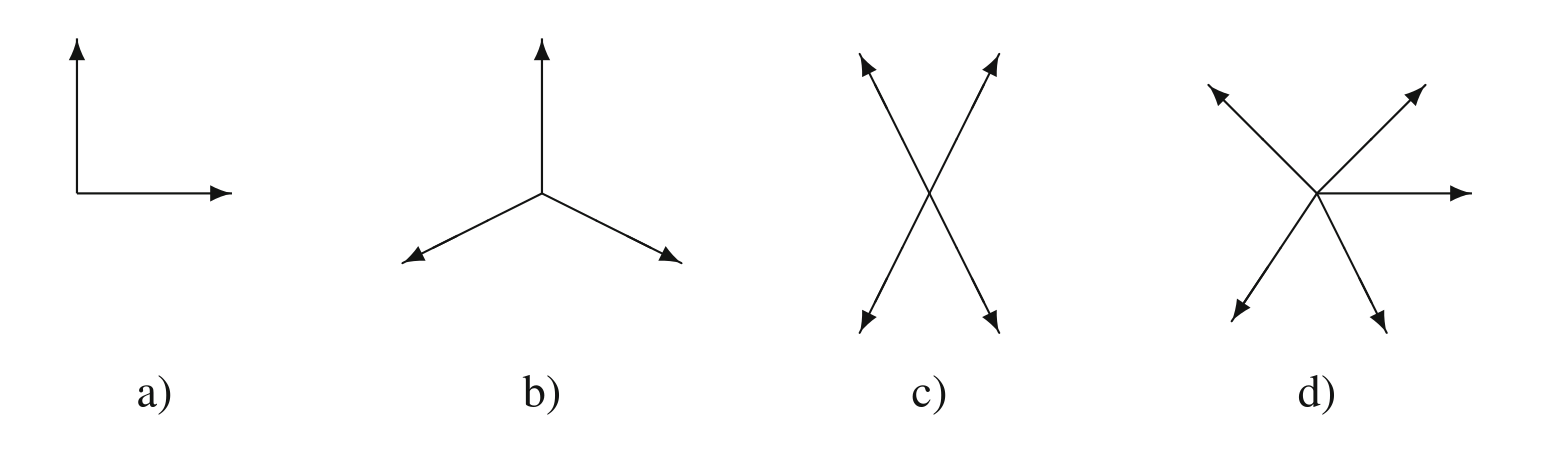
\includegraphics[width = 14cm]{illustration_pspan_pbases.png}
    \caption{Illustration d'une base (a), de 2 bases positives (b), (c) et un span positif (d) dans $\mathbb{R}^2$. Source : \cite{AuHa2017a}.}
    \label{fig:bases,pspan, pLI}
\end{figure}

Nous pouvons remarquer à cette figure que, une base positive de $\mathbb{R}^2$ ne contient pas 2 vecteurs comme c'était le cas pour une base. Elle peut en contenir 3, voir 4, et être toujours une base positive. Par contre, plus de 4 vecteurs semblent être la limite dans $\mathbb{R}^2$.  Au vu de ces exemples, on peut se demander combien de vecteurs se trouvent au minimum et au maximum dans une base positive de $\mathbb{R}^n$.
La proposition suivante va nous permettre d'obtenir une borne inférieure sur la cardinalité d'une base positive de $\mathbb{R}^n$ en s'intéressant d'abord à la cardinalité d'un ensemble générateur positif $\mathbb{R}^n$.

\proposition{Générateur positif minimal}
{
    Soit $\mathbb{D}$ un ensemble générateur positif de $\mathbb{R}^n$. Alors, $\mathbb{D}$ contient au moins $n+1$ vecteurs.
}

\preuve
{
    Si $\mathbb{D}$ contient une infinité de vecteurs, alors il contient trivialement au moins n+1 vecteurs. Par conséquent, nous considérerons $ \mathbb{D} = \{ d_1,d_2,\dots,d_m \}$. Etant donné que $\D$ est un ensemble générateur positif, et donc que $pspan(\D) = \mathbb{R}^n$, nous savons qu'il existe une combinaison linéaire positive tel que $-d_1 = \sum_{i=1}^m \lambda_i d_i$. En développant,



    \begin{align*}
        -d_1                               & = \sum_{i=1}^m \lambda_i d_i                      \\
        \Leftrightarrow -d_1               & = \lambda_1 d_1 + \sum_{i=2}^m \lambda_i d_i      \\
        \Leftrightarrow -(1+\lambda_1) d_1 & = \sum_{i=2}^m \lambda_i d_i                      \\
        \Leftrightarrow d_1                & = \sum_{i=2}^m \frac{-\lambda_i}{1+\lambda_1} d_i \\
    \end{align*}

    Etant donné que $\frac{-\lambda_i}{1+\lambda_1} \in \mathbb{R}$, $d_1$ est une combinaison linéaire des vecteurs $d_i$ avec $i=2,3,\dots,n$ et donc $d_1 \in span(\mathbb{D}\backslash \{ d_1 \})$. On obtient donc les relations
    $$
        \mathbb{R}^n = pspan(\mathbb{D}) \subseteq span(\mathbb{D} \subseteq span(\mathbb{D}\backslash \{ d_1 \}),
    $$
    et $\D \backslash \{d_1\}$ est un ensemble générateur pour $\mathbb{R}^n $. En conclusion, $\D \backslash \{d_1\} $ contient au moins n vecteur (puisque générateur de $\mathbb{R}^n$) et $\D$ contient au moins $n+1$ vecteurs.
}

\theoreme{Base positive maximale et minimale}
{
    Soit $\D$ une base positive de $\mathbb{R}^n$. Alors $\D$ a au moins $n+1$ vecteurs et au plus $2n$ vecteurs.
}
\preuve
{
    \textcolor{red}{partie 1 avec prop précédente, partie 2 : preuve à trouver (et à comprendre) fouiller linear programming "p154 derivative free and bb opti"}
}

\section{La construction d'une base positive}

Dans cette section, nous allons voir une façon simple de créer une base positive à partir d'une base. La différence de cardinalité entre une base positive maximale et minimale augmente avec la dimension de l'espace et il peut être intéressant de pouvoir construire aisément une base positive à partir d'un concept que l'on connait bien : les bases. En effet, pour créer une base de $\mathbb{R}^n$, il suffit d'avoir $n$ vecteurs linéairement indépendants et nous serons assurés que ceux-ci seront générateurs de notre espace. Plus simple encore, il suffit de prendre les $n$ vecteurs canoniques et nous aurons une base de $\mathbb{R}^n$. Malheureusement, ce n'est pas transposable aux bases positives mais on peut tout de même s'en servir.
Pour cela, nous allons définir la base positive canonique minimale et maximale.

\definition{Base positive canonique minimale}
{
    La base positive canonique minimale est
    $$\D_{min} = \{ e_1,e_2,\dots,e_n,-\sum_{i=1}^n e_i \},$$
    où $e_i$ est le i-ème vecteur de la base canonique de $\mathbb{R}^n$. Celle-ci est minimale puisqu'elle contient $n+1$ vecteurs.
}


\definition{Base positive canonique maximale}
{
    La base positive canonique maximale est
    $$\D_{max} = \{ e_1,e_2,\dots,e_n,-e_1,-e_2,\dots,-e_n \},$$
    où $e_i$ est le i-ème vecteur de la base canonique de $\mathbb{R}^n$. Celle-ci est maximale puisqu'elle contient $2n$ vecteurs.
}

Ces 2 bases positives $\mathbb{R}^n$ construites à partir de la base canonique de ce même espace sont bien des bases positives puisque ses vecteurs sont positivement linéairement indépendants par construction et générateurs de $\mathbb{R}^n$.
Afin de passer à une construction plus générale, énonçons le lemme \ref{lemme:construction base positive}.

\lemme{Construction d'une base positive}
{
    Soit $A \in \mathbb{R}^{n\ \times n}$ une matrice inversible. Étant donné un ensemble $\D \{d_1,d_2,\dots,d_m\}$, définissons $\mathbb{B} = \{Ad_1,Ad_2,\dots,Ad_m\}$.
    \begin{enumerate}
        \item Si $\D$ est un ensemble générateur positif pour $\mathbb{R}^n$, alors $\mathbb{B}$ est un ensemble générateur positif $\mathbb{R}^n$.
        \item Si $\D$ est positivement linéairement indépendant, alors $\mathbb{B}$ est positivement linéairement indépendant.
        \item Si $\D$ est une base positive de $\mathbb{R}^n$, alors $\mathbb{B}$ est une base positive de $\mathbb{R}^n$.
    \end{enumerate}
}\label{lemme:construction base positive}
\preuve
{
    \begin{enumerate}
        \item Supposons $\D$ un ensemble générateur positif pour $\mathbb{R}^n$. $\forall x \in \mathbb{R}^n $, définissons $\hat{x} = A^{-1}x \in \mathbb{R}^n$. Étant donné que $\D$ est un ensemble générateur positif, et donc que $pspan(\D) = \mathbb{R}^n$, nous savons qu'il existe une combinaison linéaire positive tel que $\hat{x} = \sum_{i=1}^m \lambda_i d_i$. Multiplions à gauche par $A$ pour obtenir
              \begin{align*}
                  x = \sum_{i=1}^m \lambda_i (A d_i) \in  pspan(\mathbb{B}).
              \end{align*}
              Par conséquent, $\mathbb{B}$ est un ensemble générateur positif pour $\mathbb{R}^n$.

        \item Supposons $\D$ un ensemble positivement linéairement indépendant. Supposons par l'absurde qu'il existe $k$ tel que
              $$
                  A d_k \in pspan(\mathbb{B}\backslash \{ A d_k \}).
              $$
              Alors, il existe une combinaison linéaire positive tel que $A d_k = \sum_{i=1, i \neq k}^m \lambda_i d_i$. Multiplions à gauche par $A^{-1}$ pour obtenir
              $$
                  d_k = \sum_{i \neq k} \lambda_i A^{-1} A d_i = \sum_{i \neq k} \lambda_i d_i.
              $$
              Cela signifie que $d_k$ peut être obtenu via des combinaisons linéaire positives de vecteurs de $\D$, cela contredit le fait que $\D$ est un ensemble positivement linéairement indépendant. Par conséquent, notre hypothèse par l'absurde est fausse : il n'existe pas d'indice $k$, $\mathbb{B}$ est donc positivement linéairement indépendant.

        \item Si $\D$ est une base positive de $\mathbb{R}^n$, alors $\D$ est un ensemble générateur positif et positivement linéairement indépendant et par 1. et 2., $\mathbb{B}$ l'est aussi et donc $\mathbb{B}$ est une base positive de $\mathbb{R}^n$.
    \end{enumerate}
}

De manière générale, nous pouvons construire une base positive de $\mathbb{R}^n$ à partir de n'importe quel base de $\mathbb{R}^n$ comme l'illustre ce théorème.


\theoreme{Construction d'une base positive maximale et minimale}
{
    Soit $\mathbb{B} = \{ d_1,d_2,\dots,d_n \}$ une base de $\mathbb{R}^n$ et
    \begin{align*}
        \mathbb{D}_{min} & = \mathbb{B} \cup \{ -\sum_{i=1}^m d_i \}, \\
        \mathbb{D}_{max} & = \mathbb{B} \cup (-\mathbb{B}).
    \end{align*}
    Alors $\D_{min}$ est une base positive minimale de $\mathbb{R}^n$ et $\D_{max}$ est une base positive maximale de $\mathbb{R}^n$.
}\label{theoreme:construction base}
\preuve
{
    Soit $\mathbb{B}_c = \{e_1,e_2,\dots,e_n\}$, la base canonique de $\mathbb{R}^n$ et définissons $\mathbb{B} = \{A e_1,A e_2,\dots,A e_n\} := \{ d_1,d_2,\dots, d_n \} $ avec $A \in \mathbb{R}^{n\ \times n}$ une matrice inversible.

    Soit $\D_{min_{c}} = \mathbb{B_c} \cup \{-\sum_{i=1}^n e_i \} = \{ e_1,e_2,\dots,e_n,-\sum_{i=1}^n e_i \}$ la base positive canonique minimale de $\mathbb{R}^n$.
    En appliquant, le lemme \ref{lemme:construction base positive} à $\D_{min_c} \cup \{-\sum_{i=1}^n e_i \}$ qui est une base positive et l'ensemble $\mathbb{B} \cup \{-\sum_{i=1}^n d_i \}$, alors ce dernier est bien une base positive qui est minimale puisqu'elle contient $n+1$ vecteurs.

    Par un raisonnement similaire, on obtient le résultat pour $\D_{max}$ à partir de la définition de base positive canonique maximale.
}

La figure \ref{fig:bases,pspan, pLI} illustre ces 2 bases. En effet, (b) est une base positive minimale alors que (c) est une base positive maximale, toutes deux obtenues via la construction proposée par le théorème \ref{theoreme:construction base}.

\section{Bases positives et direction de descente}

Dans cette section, nous allons aborder le lien entre direction de descente et base positive et finalement comprendre pourquoi travailler avec des bases positives dans les algorithmes de recherche directe est intéressant. Avant toute chose, définissons une direction de descente.

\definition{Direction de descente}
{
    Une direction $d \in  \mathbb{R}^n$ est appelée direction de descente d'une fonction $f$ au point $x \in \mathbb{R}^n$ si et seulement si il existe un réel strictement positif $\Tilde{t}$ tel que
    $$
        f(x+td) < f(x) \hspace{0.5cm} \forall t\in ]0,\Tilde{t}]
    $$
}
En d'autres termes, une direction est une direction de descente si suivre cette dernière jusqu'à un certain point diminue la valeur de notre fonction.

La notion de direction de descente est liée à la notion de dérivée directionnelle définie ci-dessous.

\definition{Dérivée directionelle}
{
    On appelle dérivée directionnelle de $f$ en $x$ dans la direction $d \in \mathbb{R}^n$ la fonction
    $$
        f'(x;d):= \lim\limits_{\substack{t \to 0 \\ t>0}}\frac{f(x+td - f(x)}{t}.
    $$
    Si $f \in \mathcal{C}^1$, alors la dérivée directionnelle satisfait
    $$
        f'(x;d) = d^T \nabla f(x) \hspace{0.5cm} \forall d \in \mathbb{R}^n.
    $$
}

Ce lien est exprimé ci-dessous.

\begin{itemize}
    \item Si $d$ est une direction de descente de $f$ en $x$, alors $f'(x;d) \leq 0$
    \item Si $f'(x;d) < 0$, alors $d$ est une direction de descente de $f$ en $d$
\end{itemize}

Finalement, le théorème ci-dessous lie base positive, direction de descente et dérivée directionnelle.

\theoreme{Base positive et direction de descente}
{
    Soit $\D$ un ensemble générateur positif dans $\mathbb{R}^n$ et $w \in \mathbb{R}_0^n$.
    Alors il existe $d \in \D$ tel que $w^T d < 0$. De plus, si $f \in \mathcal{C}^1$ et $\nabla f(x) \neq 0 $ pour au moins un $x \in \mathbb{R}^n$, alors il existe $d \in \D$ tel que $d$ est une direction de descente de $f$ en $x$.
}
\preuve
{
    Soit $\D$ un ensemble générateur positif de $\mathbb{R}^n$ avec $m$ éléments, alors il existe une combinaison linéaire positive pour obtenir $-w \in \mathbb{R}^n$ tel que
    $$
        -w = \sum_{i=1}^m \lambda_i d_i, \text{ où } d_i \in \D.
    $$
    Notons que
    $$
        0 > - ||w||^2 = -w^T w = \sum_{i=1}^m \lambda_i w^T d_i.
    $$
    Puisque $\lambda_i \geq 0 \forall i $, il est obligatoire que $w^T d_i < 0 $ pour au moins un indice $i$, et donc il existe $d \in \D$ tel que $w^T d < 0$.
    Si $\nabla f(x) \neq 0$, alors il existe un vecteur $d \in \D$ tel que $0 > \nabla f(x) ^T d = f'(x;d)$ en appliquant ce qui a été montré ci-avant. Cela implique que $d$ est  une direction de descente pour $f$ en $x$.
}

Ce théorème apporte un résultat très important puisqu'il montre qu'au moins un élément d'un ensemble générateur positif (et donc d'une base positive) est une direction de descente dès l'instant où $f \in \mathcal{C}^1$ et $\nabla f(x) \neq 0$, ce qui n'est pas toujours le cas pour un ensemble générateur. Cela signifie qu'en évaluant notre fonction $f$ dans chaque direction $d \in \D$, nous sommes assurés qu'au moins une d'entre-elles diminuera la valeur de notre fonction, ce qui est intéressant dans un problème de d'optimisation.






\chapter{Optimisation boîte-noire}

Ce chapitre concernera l'optimisation, et plus particulièrement l'optimisation boîte-noire. Après avoir défini ce concept et le problème associé, nous aborderons l'optimisation avec et sans contrainte. Le contenu textuel de ce chapitre est tiré du cours \cite{coursFranco} ainsi que l'ouvrage \cite{AuHa2017a}

\section{Les problèmes d'optimisation boîte-noire}


Nous pouvons distinguer différents problèmes d'optimisation : les problèmes utilisant des informations sur le gradient et ceux ne les utilisant pas comme illustré à la figure \ref{fig:classification_methode_opti}.

\begin{figure}[htbp]
    \centering
    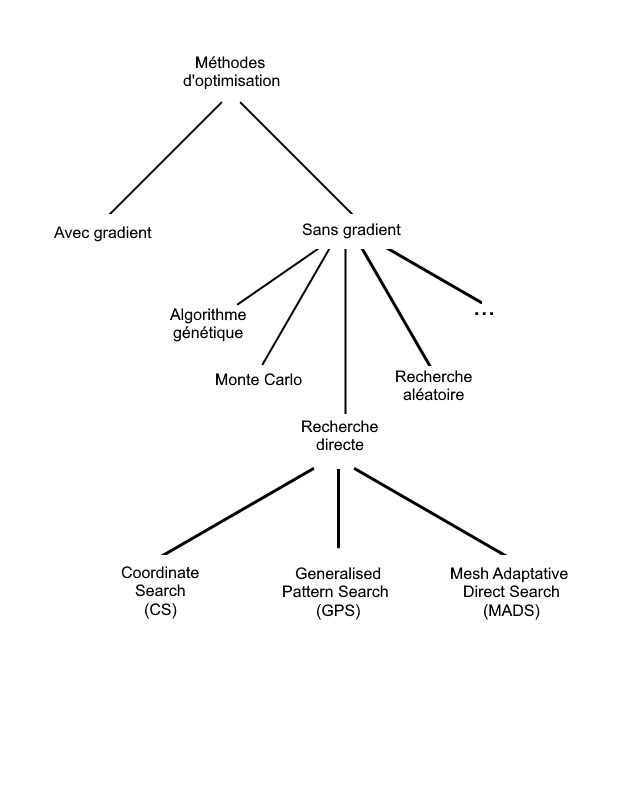
\includegraphics[width=13cm]{classification.png}
    \caption{Classification de différentes méthodes d'optimisation selon l'utilisation ou non du gradient.}
    \label{fig:classification_methode_opti}
\end{figure}

Les premiers peuvent être utilisés lorsque nous possédons l'expression du gradient et que l'évaluation de celui-ci ne demande pas trop de ressources (on peut par exemple citer l'algorithme du gradient conjugué dans cette catégorie). Néanmoins, dans certaines applications, celui-ci n'est pas utilisable et d'autres méthodes peuvent alors s'avérer utiles, voire indispensables, parmi celles-ci se trouvent les algorithmes de recherche directe que nous aborderons au chapitre \ref{chapter:direct search} et ce sont en partie ces méthodes qui seront utilisées lors de l'optimisation boîte-noire.
Dans cette section, nous allons aborder le concept de boîte-noire, l'optimisation boîte-noire ainsi que ses inconvénients et avantages.

\subsection{Le concept de boîte-noire}

Une boîte-noire est un processus qui, à partir d'une ou plusieurs entrées, crée une sortie où le lien entre les entrées et la sortie n'est pas disponible analytiquement comme l'illustre la figure \ref{fig:blackbox}. Nous pouvons voir cela comme faire la préparation d'un gâteau sans recette avec un acolyte : nous pouvons choisir une certaine quantité d'ingrédients (les entrées), donner ces ingrédients à notre acolyte qui va se charger de les associer, cuire cette association (la boîte-noire) et il va nous revenir avec un résultat (la sortie) mais le processus entre le choix des ingrédients et le résultat nous est inconnu (ou trop complexe).

\begin{figure}
    \centering
    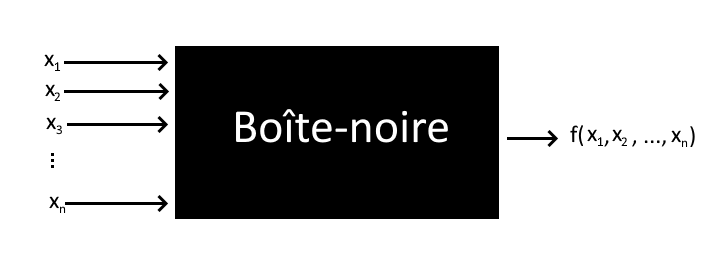
\includegraphics[width=13cm]{blackbox.png}
    \caption{Illustration du concept de boite-noire.}
    \label{fig:blackbox}
\end{figure}

\subsection{Le problème d'optimisation}

Un problème d'optimisation boîte-noire consiste à optimiser (sans perdre de généralité, nous considérerons par la suite des problèmes de minimisation) une fonction objectif, avec ou sans contraintes, où celle-ci est calculée à partir d'une sortie d'une boîte-noire. On va résoudre ce type de problème via des méthodes d'optimisation sans gradient puisque seulement la sortie de notre boîte-noire est connue et le gradient inconnu.


\begin{equation}
    \begin{aligned}
        \min_{x_i} \quad    & f(x_{i})     \\
        \textrm{s.c.} \quad & g(x_i) \geq0 \\
    \end{aligned}
\end{equation}




\section{L'optimisation sans contraintes}

\section{L'optimisation avec contraintes}






\chapter{Algorithme de recherche directe}\label{chapter:direct search}

Dans ce chapitre, nous commencerons par introduire les méthodes de recherche directe. Ensuite, nous aborderons différents algorithmes avec, en premier lieu, \textit{Coordinate Search } (CS) qui est un des plus simples algorithmes dans cette catégorie pour ensuite aborder l'algorithme \textit{General Pattern Search } (GPS) et finalement aborder le plus complexe des trois, l'algorithme \textit{Mesh Adaptative Direct Search} (MADS). Ce qui est présenté dans ce chapitre est fortement basé sur l'ouvrage \cite{AuHa2017a}.

\section{Les méthodes de recherche directe}
Les méthodes de recherche directe sont des méthodes qui, à chaque itération, évaluent un ensemble de points et mettent à jour la solution courante s'il en trouve une meilleure dans cet ensemble. Dans le cas contraire, la taille des pas est réduite. Par la suite, afin de ne pas perturber les esprits et être le plus clair possible, lorsque nous parlerons d'itération, celle-ci sera mise en exposant de la variable.

\section{Coordinate search (CS)}

L'un des plus simples algorithmes de recherche directe est appelé "coordinate search" (CS) dont le pseudo-code est disponible à l'algorithme \ref{algo::CS}. L'idée derrière cet algorithme est de rechercher à chaque itération $k$, dans les directions des vecteurs $e_i$ de la base canonique de $\mathbb{R}^n$ et à une longueur $\delta^k$ du point $x^k$, si l'on peut trouver un point $x^{k+1}$ qui améliore la valeur de la fonction objectif $f$. C'est-à-dire rechercher si on trouve un point améliorant $f$ dans l'ensemble $P^k := \{ x^k \pm \delta^k e_i : i=1,2,\dots,n\}$, l'ensemble des points situés à une distance $\delta^k$ dans les directions des vecteurs de la base canonique. Si c'est le cas, alors ce point est sauvegardé et on recommence la recherche à partir de ce point à l'itération suivante. Sinon, on divise la taille du pas par deux et on recommence la recherche à partir du même point $x^k$. Lorsque la taille du pas devient inférieure à notre critère d'arrêt $\epsilon_{stop}$, alors l'algorithme s'arrête.

\begin{algorithm}[htbp]

    \SetAlgoNoLine
    \caption{Coordinate search (CS)}
    \Entree{Une fonction $f:\mathbb{R}^n \rightarrow \mathbb{R} $ et une condition initiale $x_0 \in \mathbb{R}^n$}

    \tcp{Initialisation}

    \Indp
    $\delta^0 \in ] 0,\inf [$ \hspace{1cm} taille de pas \\
    $\epsilon_{stop} \in [ 0,\inf [$ \hspace{0.56cm} critère d'arrêt \\
    $k \leftarrow 0$ \hspace{1.73cm} itérateur \\
    \Indm

    \Indp
    \Tq{$\delta^{k+1} \geq \epsilon_{stop}$}{
        \tcp{Sondage}
        \eSi{ $\exists \hspace{2pt} t \in P^k := \{ x^k \pm \delta^k e_i : i=1,2,\dots,n\}$ tel que $f(t) < f(x_k)$}{
            $x^{k+1} \leftarrow t$ \\
            $\delta^{k+1} \leftarrow \delta^k$
        }{
            $x^{k+1} \leftarrow x^k$ \\
            $\delta^{k+1} \leftarrow \frac{1}{2}\delta^k$
        }
        $k \leftarrow k+1$
    }
    \Indm
    \label{algo::CS}
\end{algorithm}

La figure \ref{fig:CS} illustre l'algorithme dans $\mathbb{R}^2$. À l'itération 0, avec $x_0 = (2,2)$, nous évaluons les points situés à une distance $\delta_0 = 1$ dans la direction des vecteurs de la base canonique et nous trouvons que le point $(1,2)$ améliore la valeur de la fonction objectif, ce point est donc sauvegardé, $x_1=(1,2)$ et nous passons à l'itération suivante. À l'itération 1, nous répétons le même processus à partir de $x_1$ avec $\delta_1 = 1$  mais cette fois-ci, aucun point améliorant la fonction objectif n'est trouvé. Dans ce cas, nous passons à l'itération suivante avec $x_2 = x_1$ et $\delta_2 = \frac{\delta_1}{2} = \frac{1}{2}$. Nous recherchons maintenant toujours des points dans les mêmes directions mais cette-fois plus proche de la solution en cours.

\begin{figure}[htbp]
    \centering
    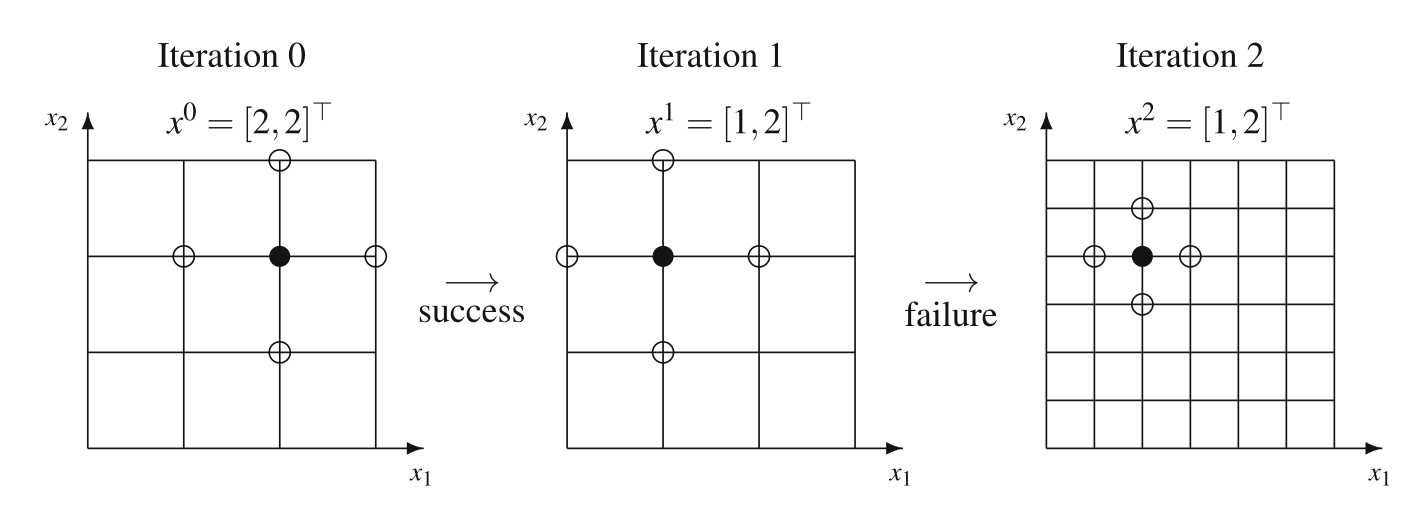
\includegraphics[width=14cm]{CS_algo_illustration.png}
    \caption{Illustration de l'algorithme CS dans $\mathbb{R}^2$. Source : \cite{AuHa2017a}.}
    \label{fig:CS}
\end{figure}

Cet algorithme présente certains problèmes,
\begin{itemize}
    \item À chaque itération, nous évaluons $2n$ points pour un problème dans $\mathbb{R}^n$. Naturellement, si la dimension du problème est grande et que chaque évaluation de la fonction en ces points est coûteuse, cela peut rapidement poser un problème pour trouver les points améliorant la fonction objectif d'itération en itération.
    \item La méthode d'optimisation est plutôt locale que globale. En effet, l'algorithme ne s'autorise jamais à explorer à une distance au-delà de la longueur du pas initial : soit elle diminue, soit elle reste constante mais jamais elle n'augmente. Cela signifie, que si notre algorithme est coincé dans un minimum local, il ne pourra pas s'échapper de celui-ci. De ce fait, la méthode est fortement dépendante de la condition initiale.
    \item Le sondage de l'espace se fait toujours dans les mêmes directions d'itérations en itérations et ces directions sont toujours celles suivant les vecteurs de la base canonique. Cependant, ces directions ne sont pas choisies pour être optimales et on peut imaginer que, sur le grillage parcouru par notre algorithme comme l'illustre la figure \ref{fig:CS}, si la direction idéale est sur une diagonale, on va devoir avancer en zig-zag pour la suivre et donc perdre de précieuses itérations comparé au fait de suivre directement cette direction.
\end{itemize}





\section{Generalised Pattern Search (GPS)}

L'algorithme précédent n'est clairement pas idéal mais il présente des similitudes avec l'algorithme dont nous allons parler dans cette section et nous utiliserons les concepts abordés dans le chapitre \ref{chapter:Bases positives}.

\definition{Maillage}
{
    Soit $G \in \mathbb{R}^{n \times n}$ inversible et $Z \in \mathbb{Z}^{n \times p}$, $(p > n)$ tel que les colonnes de $Z$ forment un ensemble générateur positif de $\mathbb{R}^n$. Définissons $D=GZ$. Le maillage de taille uniforme $\delta^k > 0$ généré par $D$ centré en $x^k \in \mathbb{R}^n$ est défini par
    $$
        M^k := \{ x^k + \delta^k D y : y \in \mathbb{N}^p \} \subset \mathbb{R}^n
    $$
    $\delta^k$ est le paramètre de taille du maillage.
}

Les colonnes de la matrice $Z$ forment un ensemble générateur positif de $\mathbb{R}^n$ et $G$ est une matrice inversible et donc, par le lemme \ref{lemme:construction base positive}, les colonnes de $D=GZ$ forment un ensemble générateur positif de $\mathbb{R}^n$.

Soit $\D$ un ensemble de directions dans $\mathbb{R}^n$, composé des colonnes de $D$. Cet ensemble $\D$ sera l'ensemble des directions d'explorations possibles de l'algorithme GPS qui peuvent être beaucoup plus variées que dans l'algorithme CS où les directions d'explorations étaient les directions (positives et négatives) des vecteurs canoniques.

Présentons l'algorithme  GPS \ref{algo::GPS} pour un problème de minimisation sans contrainte.

\begin{algorithm}[htbp]

    \SetAlgoNoLine
    \caption{Generalised pattern search (GPS)}
    \Entree{Une fonction $f:\mathbb{R}^n \rightarrow \mathbb{R} $ et une condition initiale $x_0 \in \mathbb{R}^n$}

    \tcp{Initialisation}

    \Indp
    $\delta^0 \in ] 0,\inf [$ \hspace{40pt} taille initiale du maillage \\
            $D=GZ$ \\
            $\tau \in ]0,1[ \in \mathbb{R}$ \hspace{35pt} paramètre de taille du maillage

    $\epsilon_{stop} \in [ 0,\inf [$ \hspace{28pt} critère d'arrêt \\
    $k \leftarrow 0$ \hspace{61pt} itérateur \\
    \Indm


    \Indp
    \Tq{$\delta^{k+1} \geq \epsilon_{stop}$}{
        \tcp{Recherche}

        \eSi{$\exists \hspace{2pt} t \in S^k \subseteq M^k$ tel que $f(t) < f(x^k)$ }
        {
            $x^{k+1} \leftarrow t$ \\
            $\delta^{k+1} \leftarrow \tau^{-1} \delta^k$
        }
        {
            \tcp{Sondage}
            choisir un ensemble générateur positif $\mathbb{D}^k \subseteq \mathbb{D}$ \\
            \eSi{$\exists \hspace{2pt} t \in P^k := \{ x^k + \delta^k d : d \in \mathbb{D}^k\}$ tel que $f(t) < f(x^k)$ }
            {
                $x^{k+1} \leftarrow t$ \\
                $\delta^{k+1} \leftarrow \tau^{-1} \delta^k$
            }{
                $x^{k+1} \leftarrow x^k$ \\
                $\delta^{k+1} \leftarrow \tau \delta^k$
            }
        }


        $k \leftarrow k+1$
    }
    \Indm
    \label{algo::GPS}
\end{algorithm}

Après l'initialisation, nous pouvons distinguer 2 grandes étapes au cours d'une itération de l'algorithme : la phase de recherche et la phase de sondage. Explicitons chacune de ces étapes.

La phase de recherche, qui n'était pas présente dans l'algorithme CS, permet de résoudre le problème d'optimisation locale dans celui-ci. En effet, à chaque itération, l'algorithme s'autorise à sélectionner et évaluer un nombre fini de points du maillage $M^k$. Nous sommes libres de choisir le nombre de points sélectionnés (tout en gardant à l'esprit qu'il faut évaluer chaque sélection) et de les choisir éloignés ou non de notre solution courante $x^k$. De ce fait, notre algorithme va pouvoir sortir d'un minimum local s'il sélectionne et évalue un meilleur point lors de la phase de recherche. La façon de sélectionner est libre, on peut imaginer sélectionner un certain nombre de points au hasard à chaque itération.

Dans le cas où la phase de recherche échoue, la phase de sondage débute. Cette phase de sondage est similaire à celle présente dans l'algorithme CS dans le sens où nous cherchons des points à une distance $\delta^k$ de la solution courante $x_k$ dans certaines directions et améliorant la fonction objectif. Les changements se situent dans un premier temps au niveau des directions, celles-ci sont dorénavant choisies parmi un ensemble générateur positif $\D$ et seulement dans une direction positive, ce choix offre plus de flexibilité et de variabilité (puisque $\D^k$ peut changer à chaque itération). Si parmi les points évalués dans ces directions à une distance $\delta^k$, nous en trouvons un améliorant la fonction $f$, alors nous le conservons pour l'itération suivante et la taille du maillage augmente d'un facteur $\tau^{-1}$ supérieur à 1 (afin d'accélérer la convergence vers le minimum d'itération en itération et compenser un potentiel mauvais choix pour la valeur de $\delta^0$). Dans le cas contraire, nous conservons la solution courante, diminuons la taille du maillage d'un facteur $\tau$ entre 0 et 1 (afin d'être plus précis dans notre sondage lors de l'itération suivante) et passons à l'itération suivante.

Finalement, abordons le dernier changement : l'initialisation de $D = G Z$. En effet, $\D$ est un ensemble générateur positif composé des colonnes de $D$ parmi lequel nous sélectionnons les directions à chaque itération. Il peut être intéressant de se demander quel est l'impact de ces 2 matrices $G$ et $Z$. La première va impacter la structure du maillage comme l'illustre la figure \ref{fig:GPS GZ}, la matrice identité va créer un maillage avec une structure composée de carrés alors que la matrice utilisée pour (c) crée un maillage triangulaire. La matrice $Z$ va quant à elle se charger des directions, chaque colonne en est une, comme l'illustre cette même figure \ref{fig:GPS GZ}.

\begin{figure}[htbp]
    \centering
    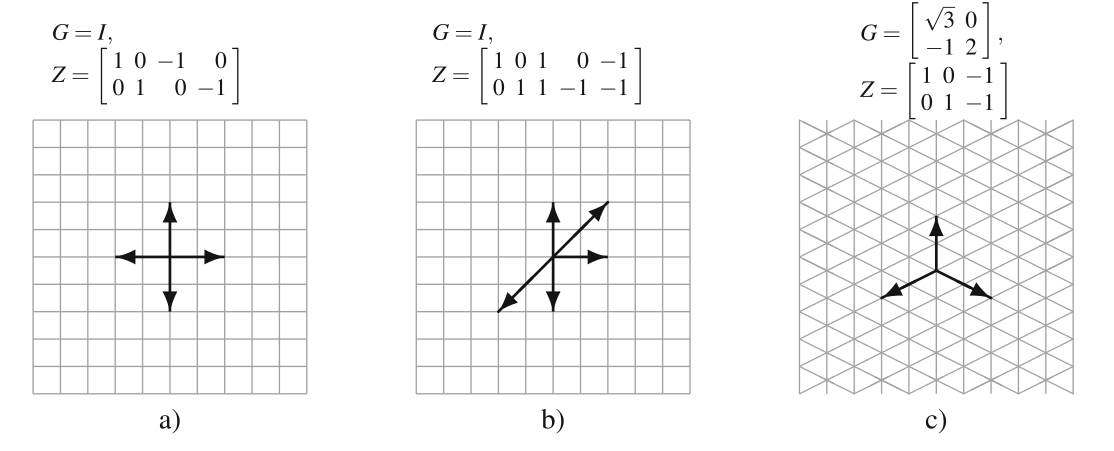
\includegraphics[width=12cm]{GPS_GZ.png}
    \caption{Représentation de l'impact des matrices $G$ et $Z$ dans $\mathbb{R}^2$ avec $\delta^k=\frac{1}{2}$ sur la structure du maillage et l'ensemble des directions de $\D$. Source : \cite{AuHa2017a}.}
    \label{fig:GPS GZ}
\end{figure}

Remarquons que si $G$ est la matrice identité et que les colonnes de $Z$ sont les vecteurs positifs et négatifs de la base canonique, alors CS et GPS ont la même phase de sondage (à la différence près que $\delta^k$ peut augmenter dans le second cas). Nous pouvons voir que pour (b), les colonnes de $Z$ ne sont pas positivement linéairement indépendantes et ne forment donc pas une base de $\mathbb{R}^2$ contrairement à (a) et (c). Le fait que les colonnes forment un ensemble générateur positif suffit et ce surplus peut même être un avantage puisque $\D^k$ va pouvoir changer à chaque itération et ainsi apporter plus de flexibilité et variabilité. Rappelons que $\D^k$ doit être générateur positif.

Finalement, le maillage n'est en pratique pas construit entièrement sinon nous perdrions tout l'intérêt de l'optimisation puisqu'il faudrait évaluer tous les points du maillage. Cependant, nous nous déplaçons dessus localement et surtout, il est utile pour comprendre le fonctionnement de l'algorithme.

\section{Mesh Adaptative Direct Search (MADS)}
L'algorithme mesh adaptative direct search (MADS) est un algorithme permettant de résoudre des problèmes d'optimisation avec et sans contrainte. L'algorithme, en plus d'utiliser un maillage (ainsi qu'un paramètre $\delta^k$ ajustant sa taille), celui-ci utilise également un cadre (ainsi qu'un paramètre d'ajustement $\Delta^k$) que nous définissons ci-dessous.

\definition{Cadre}
{
    Soit $G \in \mathbb{R}^{n \times n}$ inversible et $Z \in \mathbb{Z}^{n \times p}$, $(p > n)$ tel que les colonnes de $Z$ forment un ensemble générateur positif de $\mathbb{R}^n$. Définissons $D=GZ$.
    Soit $\Delta^k$, le paramètre de taille du cadre tel que $\Delta^k \geq \delta^k > 0$.
    Le cadre généré par $D$, centré en $x^k \in \mathbb{R}^n$, est défini par
    $$
        F^k := \{ x\in M^k : || x-x^k ||_\infty \leq \Delta^k b \}
    $$
    avec $M^k$, le maillage à l'itération $k$, $b = max\{ || d' ||_\infty : d' \in \D \}$ et $\Delta^k$ est le paramètre de taille du cadre.
}

Notons que $F^k \subseteq M^k$.
Afin de comprendre l'intérêt de ces 2 concepts, illustrons-les dans $\mathbb{R}^2$.

Soit
$$
    D=\begin{pmatrix}
        1 & 0 & 1 & 1  & -1 & 0  & -1 & -1 \\
        0 & 1 & 1 & -1 & 0  & -1 & -1 & 1
    \end{pmatrix}
$$
La figure \ref{fig:MADS illustration} illustre différents maillages en trait fin (de paramètre de taille $\delta^k$) et différents cadres en trait noir (de paramètre de taille $\Delta^k$) ainsi que 3 points sondés $p^1,p^2,p^3$. Dans le premier exemple en haut à gauche, $\delta^k = \Delta^k = 1$ et 3 points ont été sélectionnés parmi les 8 possibles (à l'intérieur ou à l'intersection du cadre et du maillage hormis le point $x_k$ naturellement). Dans tous les autres cas, $\delta^k < \Delta^k$ et le nombre de points que l'on peut sonder augmente. Lorsque $\delta^k=\frac{1}{4}$ et $ \Delta^k = \frac{1}{2}$, l'algorithme a le choix parmi 24 points. En bas à gauche et à droite, celui-ci a le choix parmi 80 et 288 points respectivement. De manière générale, si $\delta^k = \frac{1}{2^p}$ et $\Delta^k = \frac{1}{4^p}$ avec $p \in \mathbb{N}$, alors nous aurons $(2^{p+1} +1)^2 -1$ choix de points du maillage.

Ceci illustrait la première différence avec GPS. Dans celui-ci, nous serions obligés de nous trouver sur le cadre à chaque itération, ce que MADS ne contraint pas en permettant de se trouver à l'intérieur du cadre et ainsi offrir un plus large éventail de points possible lors de la phase de sondage. De plus, afin de mettre à jour la taille du maillage, $\delta^k = min \{ \Delta^k,(\Delta^k)^2 \}$ et celle-ci décroit plus vite que celle du cadre, ce qui accentue le large choix de points lors de la phase de sondage d'itération en itération.

C'est pourquoi il est possible de choisir une matrice plus simple pour $D$ tel
$$
    D=\begin{pmatrix}
        1 & 0 & -1 \\
        0 & 1 & -1
    \end{pmatrix}.
$$ Cette matrice fournit le même maillage et le même cadre que la matrice $$
    D=\begin{pmatrix}
        1 & 0 & 1 & 1  & -1 & 0  & -1 & -1 \\
        0 & 1 & 1 & -1 & 0  & -1 & -1 & 1
    \end{pmatrix}
$$ donnée plus haut et illustrant la figure \ref{fig:MADS illustration}.


\begin{algorithm}[htbp]

    \SetAlgoNoLine
    \caption{Mesh adaptative Direct search (MADS)}
    \Entree{Une fonction $f_\Omega:\mathbb{R}^n \rightarrow \mathbb{R} $, une condition initiale $x_0 \in \mathbb{R}^n$}

    \tcp{Initialisation}

    \Indp
    $\Delta_0 \in ] 0,\inf [$ \hspace{40pt} taille initiale du cadre \\
            $D=GZ$ \\
            $\tau \in ]0,1[ \in \mathbb{Q}$ \hspace{38pt} paramètre de taille du maillage

    $\epsilon_{stop} \in [ 0,\inf [$ \hspace{32pt} critère d'arrêt \\
    $k \leftarrow 0$ \hspace{65pt} itérateur \\
    \Indm


    \Indp
    \Tq{$\delta_{k+1} \geq \epsilon_{stop}$}{
        \tcp{Mise à jour de $\delta_k$}
        $\delta_k = min\{ \Delta_k,(\Delta_k)^2 \}$

        \tcp{Recherche}

        \eSi{$\exists \hspace{2pt} t \in S^k \subseteq M^k$ tel que $f_\Omega(t) < f_\Omega(x_k)$}
        {
            $x_{k+1} \leftarrow t$ \\
            $\Delta_{k+1} \leftarrow \tau^{-1} \Delta_k$
        }
        {
            \tcp{Sondage}
            choisir un ensemble générateur positif $\mathbb{D}^k_\Delta $ tel que $P_k := \{ x_k + \delta_k d : d \in \mathbb{D}^k_\Delta \} \subseteq F^k$\\
            \eSi{$\exists \hspace{2pt} t \in P_k $ tel que $f_\Omega(t) < f_\Omega(x_k)$ }
            {
                $x_{k+1} \leftarrow t$ \\
                $\Delta_{k+1} \leftarrow \tau^{-1} \Delta_k$
            }{
                $x_{k+1} \leftarrow x_k$ \\
                $\Delta_{k+1} \leftarrow \tau \Delta_k$
            }
        }


        $k \leftarrow k+1$
    }
    \Indm
    \label{algo::MADS}
\end{algorithm}


\begin{figure}
    \centering
    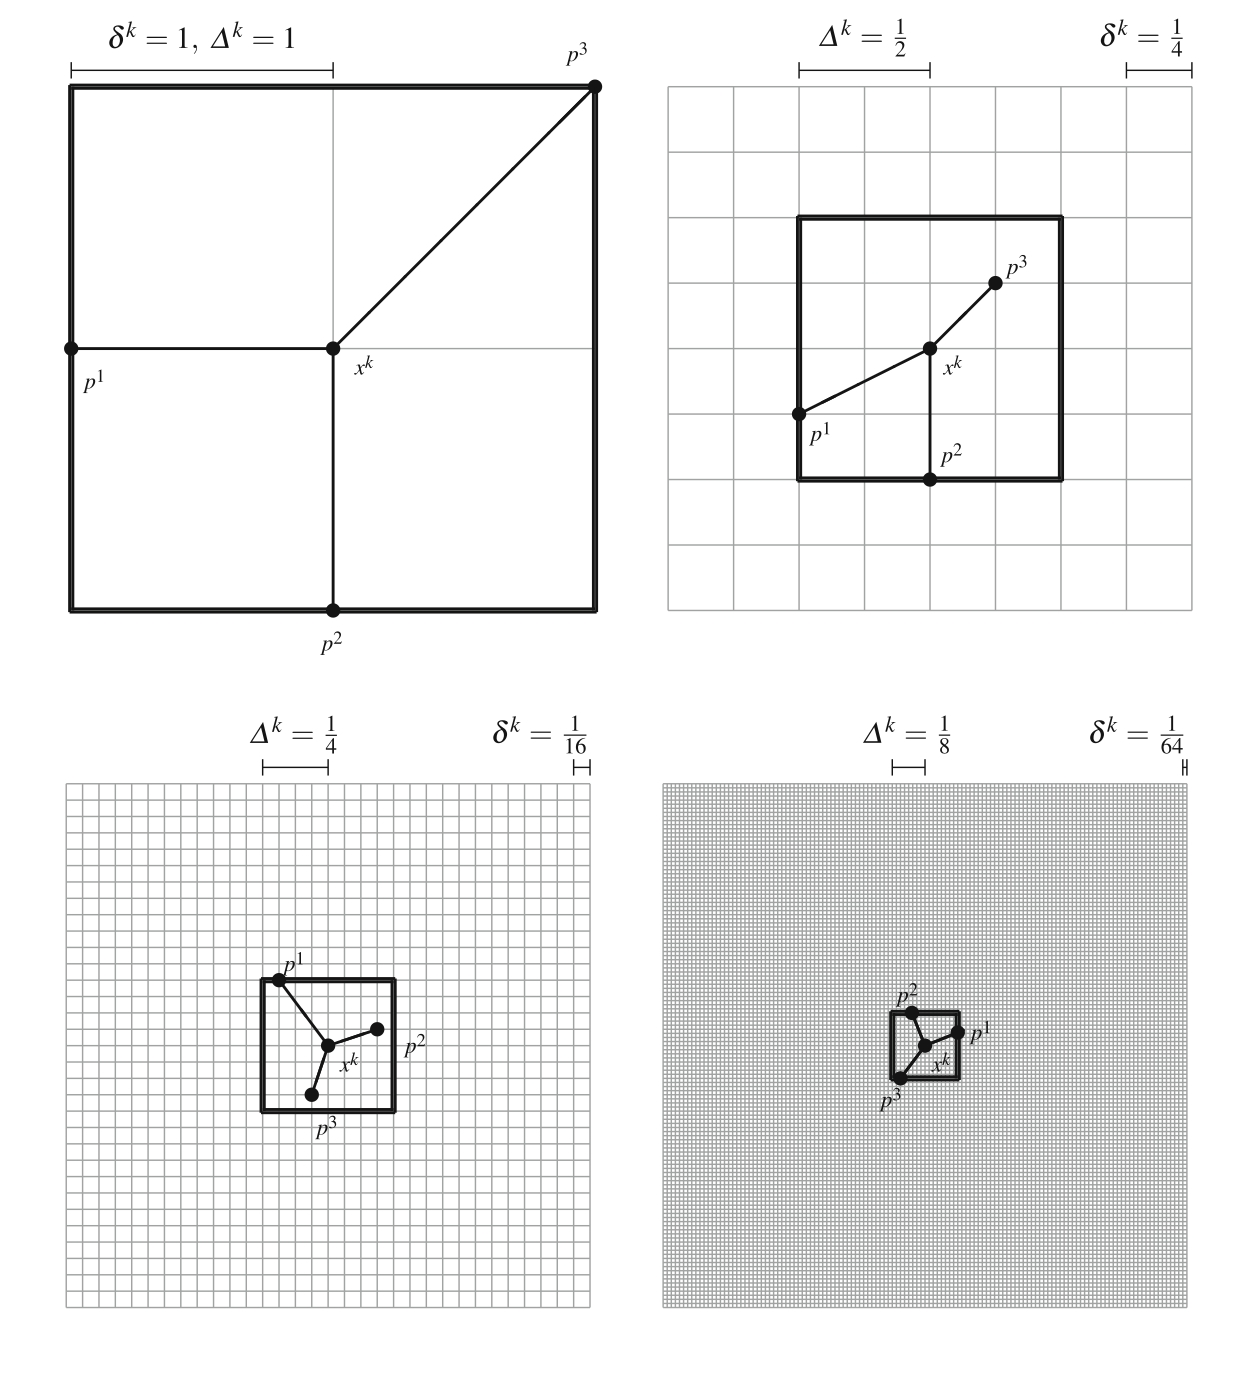
\includegraphics[width=13cm]{MADS_illustration.jpg}
    \caption{Illustration du maillage et du cadre selon différentes valeurs du paramètre de taille de maillage $\delta^k$ et de cadre $\delta^k$. Source : \cite{AuHa2017a}.}
    \label{fig:MADS illustration}
\end{figure}




\chapter{Modèles compartimentaux}

\chapter*{Conclusion}
\addcontentsline{toc}{chapter}{Conclusion}


\bibliographystyle{apalike2}
\bibliography{sources}


\end{document}
